\documentclass{article}

\usepackage[utf8x]{inputenc}
\usepackage[spanish]{babel}
\usepackage[margin=3.1cm]{geometry}
\usepackage{amsmath}
\usepackage{amssymb}
\usepackage{graphicx}
\usepackage{algorithm}
\usepackage{algorithmic}

\usepackage{ upgreek }

\usepackage{listings}

\linespread{1.2}

\title{ Computación Concurrente \\ \Large{Tarea 6}
\author{
  Diego Goméz Montesinos
  \and
  José Emiliano Cabrera Blancas
  }
\date{20 marzo 2014}
}
\begin{document}
\maketitle
\begin{enumerate}
  
  \item{
    \textsl{
      Leer y escribir un resumen de no más de 3 páginas: Given Tables
      but No Teachers, Ethiopian Children Teach Themselves, en MIT
      Technology Review, by David Talbot on October 29, 2012\\
      http://www.technologyreview.com/news/506466/given-tables-but-not-teachers-ethiopian-children-teach-themselves.\\
    } 

    ``Una laptop por niño'', u OLPC (por sus siglas en inglés, ``Once
    Laptop Per Child''),  es una organización que regala
    computadoras de bajo costo a escuelas para el apoyo de la
    educación  tecnológica a países en desarrollo.\\\\
    Esta organización realizó un experimento: regaló tablets a niños
    de las comunidades etiopes Wonchi y Wolonchete, que no saben leer,
    ni escribir, y que nunca han usado una tablet.\\
    Las tablets venían pre-cargadas con contenido educativo, y se puso
    un sistema de carga eléctrica solar.\\\\
    El experimento inició cuando los investigadores de la organización
    dejaron cajas cerradas con las tablets dentro,
    y los niños lograron encontrar, en menos de 10 minutos, la manera
    de encender los dispositivos.\\
    Después de algunos meses, los investigadores se percataron de que
    los niños  habían podido activar la webcam
    y habían modificado la apariencia del escritorio de la tablets,
    aunque ambas funcionalidades vinieran
    desactivadas por defecto.\\
    Al respecto, Ed McNierney, el jefe de tecnología de la OLPC, dice:
    ``El hecho de que hayan logrado esto
    es claramente producto de la capacidad creativa, de la capacidad
    de la curiosidad  y de la capacidad del
    descubrimiento que nosotros pensamos escenciales para el aprendizaje''.\\
    Esto abre un nuevo paradigma en la enseñanza, según la OLPC, que
    es hacer que los niños sin ningúna instrucción
    empiecen a aprender con el solo hecho de motivar la curiosidad y
    la creatividad.\\\\
    McNierney concluye: ``¿Podríamos darle a niños que no van a la
    escuela herramientas para aprendizaje sin
    proveerles escuelas, maestros y libros de texto?''.\\\\
  }
  
  \item{
      \textsl{
    Sea $\mathcal{S}$ un conjunto de simplejos en $\mathcal{A}$ un
    complejo tal que $\mathcal{S}$ $\in$ $\mathcal{A}$. Investiga las
    definiciones formales, describe cada una con tus propias palabras
    e incluye las referencias consultadas:
    }
    \begin{itemize}
      
    \item{
          \[
           Stº(\mathcal{S}, \mathcal{A}) =  \bigcup_{\mathcal{S}
             \subseteq \tau} Int \tau 
          \]

          Donde $Int\tau$ es el interior de los simplejos $\tau$.\\\\
          Podemos pensar que la operación $open$ $star$ de un simplejo
          $\mathcal{S}$ es la union de
          todos los simplejos $\tau$ que contienen a $\mathcal{S}$
          tal que le quitamos la frontera a los simplejos $\tau$
          (como si fueran intervalos abiertos).
      }
      
    \item{
        \[
           St(\mathcal{S}, \mathcal{A}) =  \bigcup_{\mathcal{S}
             \subseteq \tau} \tau 
           \]
           Intuitivamente podemos ver que la operación $star$ de un
           simplejo $\mathcal{S}$ es igual que la operación $open$
           $star$ pero sin quitarle la frontera a los simplejos
           $\tau$(como si fueran intervalos cerrados).
         }

    \item{
        \[
        Lk(\mathcal{S}, \mathcal{A}) = Dl(\mathcal{S},\mathcal{A}) \cap
        St(\mathcal{S}, \mathcal{A})
        \]
        Es el subcomplejo de $\mathcal{A}$ que consiste de todos los
        simplejos en $St(\mathcal{S},\mathcal{A})$ que no tienen
        vertices en común con $\mathcal{S}$.
      }

    \item{
        \[
        Dl(\mathcal{S},\mathcal{A})
        \]
        La operación $deletion$ de $\mathcal{S}$ $\in$ $\mathcal{A}$
        es el sucomplejo de $\mathcal{A}$ que consiste de todos los
        simplejos que no tienen vertices en común con $\mathcal{S}$.
        }
    \end{itemize}

  
  }

\item{
    \textsl{
      Realiza las operaciones y muestra de manera geométrica el
      complejo inicial y el resultante después de aplicar la operación.
      Además indica las dimensiones de los simplejos contenidos en el
      complejo resultante.
    }

    \begin{itemize}
    \item{
        \textsl{
          Sea $\mathcal{K}$ $=$ $\{\{\}, \{0\}, \{1\}, \{2\}, \{3\},
          \{0,1\}, \{0,2\}, \{1,2\}, \{1,3\}, \{2,3\}, \{0,1,2\},
          \{1,2,3\} \}$ y sea $\tau$ $=$ $\{0,1\}$. $Dl(\tau,\mathcal{K})$
        }\\
       
        El complejo inicial es:
        \begin{center}
          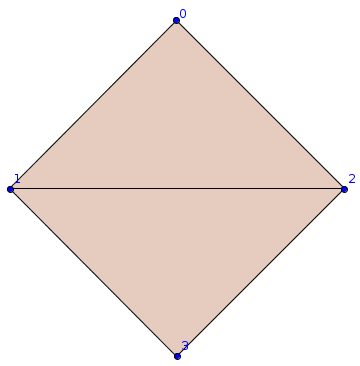
\includegraphics[scale=0.4]{entrada3_1.png}
          \\ $\mathcal{K}$
        \end{center}
        Ahora aplicando, eliminamos a los simplejos: $\{0\}, \{1\}, \{0,1\},
        \{0,2\}, \{1,2\}, \{1,3\}, \{2,3\}, \{0,1,2\},
        \{1,2,3\}$ ya que todos ellos comparten vértices con $\tau$, que son
        $\{0\}, \{1\}$. Por lo tanto la operación da como resultado el complejo:
        \begin{center}
          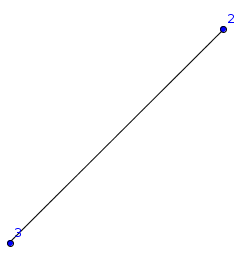
\includegraphics[scale=0.4]{salida3_1.png}
          \\ $Dl(\tau,\mathcal{K})$
        \end{center}
        El complejo resultante $Dl(\tau,\mathcal{K}) = \{\{\}, \{2\}, \{3\}, \{2,3\}\}$,
        de dimensión $-1, 0, 0$ y $1$ respectivamente.
      }
      
    \item{
        \textsl{
        Sea $\mathcal{K}$ $=$ $\{\{\}, \{0\}, \{1\}, \{2\}, \{3\},
        \{0,1\}, \{0,2\}, \{0,3\}, \{1,2\}, \{1,3\}, \{2,3\}, \{0,1,3\},
        \{0,2,3\}, \{1,2,3\}\}$ y sea $\tau$ $=$ $\{3\}$. $Lk(\tau,\mathcal{K})$
      }\\

      El complejo inicial es:
      \begin{center}
        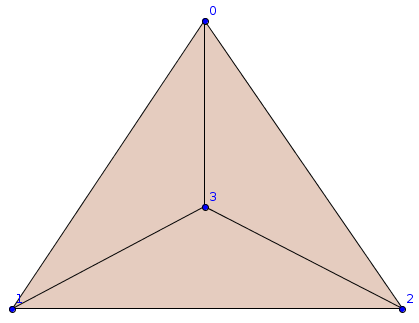
\includegraphics[scale=0.4]{entrada3_2.png}
        \\ $\mathcal{K}$
      \end{center}
      Claramente podemos ver que $\mathcal{K} = St(\tau,\mathcal{K})$, entonces
      el resultado de la operación es:
      \begin{center}
        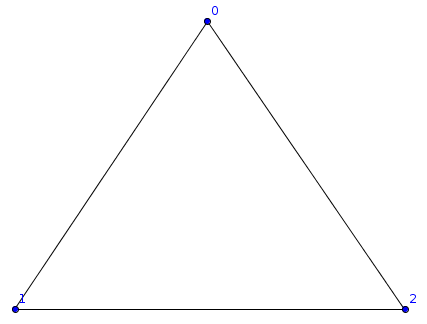
\includegraphics[scale=0.4]{salida3_2.png}
        \\ $Lk(\tau,\mathcal{K})$
      \end{center}
      El complejo resultante $Lk(\tau,\mathcal{K}) = \{\{\}, \{0\}, \{1\}, \{2\}, $
      $\{0,1\}, \{0,2\}, \{1, 2\}\}$, de dimensión $-1, 0, 0, 0, 1, 1$ y $1$ respectivamente.
    }

    \item{
        \textsl{
          Sea $\mathcal{K}$ $=$ $\{ \{ \}, \{0\} , \{1\}, \{2\}, \{3\}, \{0, 1\},\{0,
              2\}, \{0, 3\},\{1, 2\}, \{1, 3\}, \{2, 3\},
              \{0,1,3\},\{0,2,3\},\{1,2,3\}\}$ y sea $\tau$ $=$ $\{0\}$. $St(\tau,\mathcal{K})$
        }
        El complejo inicial es el mismo que el inciso anterior:
        \begin{center}
          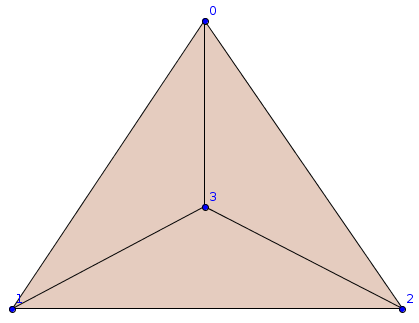
\includegraphics[scale=0.4]{entrada3_2.png}
          \\ $\mathcal{K}$
        \end{center}
        De la figura claramente podemos ver que el resultado es:
        \begin{center}
          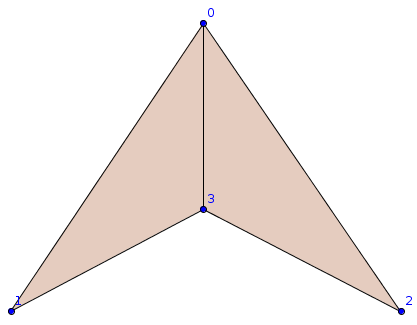
\includegraphics[scale=0.4]{salida3_3.png}
          \\ $St(\tau,\mathcal{K})$
        \end{center}
        El complejo resultante $St(\tau,\mathcal{K}) = \{\{\},\{0\},\{1\},\{2\},\{3\}, \{0,1\}, \{0,2\},
        \{0,3\}, \{1,3\}, \{2,3\},$\\ $\{0,1,3\},\{0,2,3\}\}$, de dimensión $-1, 0, 0, 0, 0, 1, 1, 1, 1,
        1, 2,$ y $2$ respectivamente.
      }

    \item{
        \textsl{
          Sea $\mathcal{K}_1$ $=$
          $\{\{\},\{0\},\{1\},\{2\},\{0,1\},\{0,2\},\{1,2\},\{0,1,2\}\}$
          y sea $\mathcal{K}_2$ $=$ $\{\{3\}, \{4\}, \{3,
          4\}\}$. $\mathcal{K}_1$ $*$ $\mathcal{K}_2$
        }
        Los complejos iniciales son:
        \begin{center}
          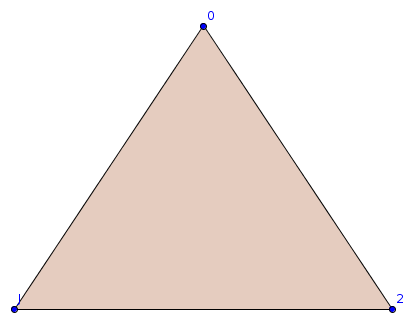
\includegraphics[scale=0.4]{entrada3_4a.png}
          \\ $\mathcal{K}_1$
        \end{center}

        \begin{center}
        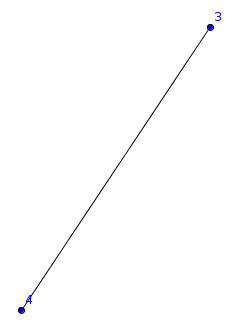
\includegraphics[scale=0.4]{entrada3_4b.png}
        \\ $\mathcal{K}_2$
        \end{center}
        El resultado del join es:
        \begin{center}
          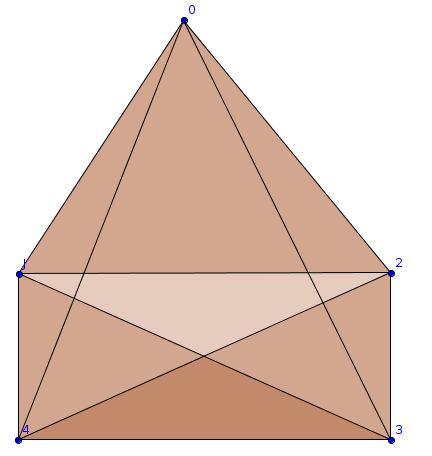
\includegraphics[scale=0.4]{salida3_4.png}
          \\  $\mathcal{K}_1$ $*$ $\mathcal{K}_2$
        \end{center}
        El complejo resultante es $\mathcal{K}_1$ $*$ $\mathcal{K}_2 = \{\{\},\{0\},\{1\},\{2\},\{3\},\{4\},\{0,1\},\{0,2\},\{1,2\},\\
        \{3,4\},\{0,3\},\{0,4\},\{1,3\},\{1,4\},\{2,3\},\{2,4\},\{0,1,2\},\{0,3,4\},\{1,3,4\},\{0,1,3\}, \\
        \{2,3,4\},\{0,2,4\}\}$, de dimensión $-1, 0, 0, 0, 0, 0, 1, 1, 1, 1, 1, 1, 1, 1, 1, 1, 2, 2, 2, 2, 2$ y $2$ respectivamente.
      }
    \end{itemize}
  }

  \item{
      \textsl{
        Demuestra que un modelo cromático tiene el mismo poder de
        cómputo que un modelo anónimo, es decir, todas las tareas
        anónimas, $\langle\mathcal{I},\mathcal{O},\Delta\rangle$ tal
        que $\mathcal{I}$ y $\mathcal{O}$ no tiene colores, que se
        pueden resolver en un modelo anónimo también las puede
        resolver un modelo cromático y viceversa.\\
        Considera modelos para tres procesos, iterado y wait-free.\\
      }
      La idea de la demostración es dada la tarea $\mathcal{T}$ en el
      modelo anónimo, debemos dar una serie de mapeos que conviertan
      la tarea $\mathcal{T}$ a una tarea $\mathcal{T}'$ en el modelo
      cromático y al final con construir una $\delta'$ que resuelva la
      tarea $\mathcal{T}'$.\\
      \\
      Demostración:\\
      Sea $\mathcal{T}$ una tarea definida por
      $\langle\mathcal{I},\mathcal{O},\Delta\rangle$ con $\mathcal{I}$
      y $\mathcal{O}$ gráficas anónimas. Por hipótesis decimos que
      existe una $\delta$ mapeo portador tal que resuelve la tarea
      $\mathcal{T}$. Primero debemos dar la tarea $\mathcal{T}'$
      definida por $\langle\mathcal{I}',\mathcal{O}',\Delta'\rangle$
      tal que es la representación de la tarea $\mathcal{T}$ en el
      modelo crómatico. \\
      Para esto vamos a definir $\Phi$ $:$ $\mathcal{G}$
      $\xrightarrow{}$ $\mathcal{G}'$ de la siguiente forma:\\

      \begin{itemize}
        
        \item{
            $\Phi(v_i) = \{\{v_{ia}, v_{ib}, v_{ic}\}\}$
          }

          \item{
              $\Phi({v_i,v_j}) =  \{\{v_{ia}, v_{ib}, v_{ic}\},
              \{v_{ja}, v_{jb}, v_{jc}\}, \{v_{ia}, v_{jb}, v_{ic}\},
              \{v_{ia}, v_{jb}, v_{jc}\}, $\\
              $\{v_{ia}, v_{ib}, v_{jc}\},
              \{v_{ja}, v_{jb}, v_{ic}\}, \{v_{ja}, v_{jb}, v_{ic}\},
              \{v_{ja},v_{ib}, v_{ic}\}
              \}$ \\
            }
        
      \end{itemize}

      La función $\Phi$ parece ser muy complicada, pero lo podemos ver
      de la siguiente forma, $\Phi$ recibe como entrada un
      subcomplejo de $\mathcal{G}$, tal que si este es un vértice que
      representa el conjunto de procesos con entrada $v_i$, $\Phi$ lo
      mapea hacia un complejo que es un triangulo relleno que tiene
      como vértices procesos con colores diferentes(a, b y c), pero con la misma
      entrada. Por otro lado si $\Phi$ recibe como un entrada una
      arista del $\mathcal{G}$, entonces la mapea a un subcomplejo que
      representa todas las combinaciones de tres procesos con dos
      posibles entradas diferentes.\\ Por definición podemos ver que
      $\Phi$ es un mapeo portador, por que tiene la propiedad de ser monotona.
      
      
      \begin{center}
        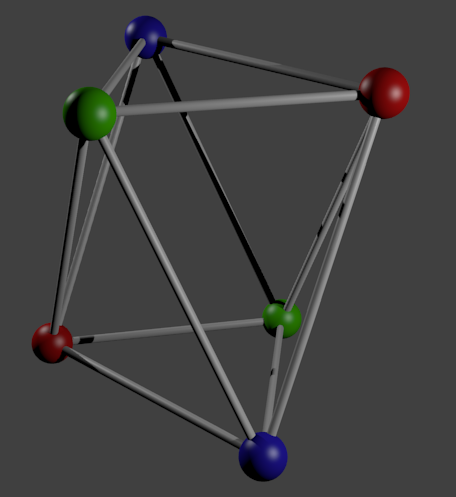
\includegraphics[scale=0.4]{phi_map.png}
        \\Complejo que resulta cuando la función $\Phi$ recibe una
        arista de entrada(es importante notar que las caras de este
        complejo deben estar rellenas).\\
      \end{center}
    
      Ahora que ya tenemos definida $\Phi$, podemos usarla para
      obtener $\mathcal{I}'$ y $\mathcal{O}'$. Simplemente pasandole a
      $\Phi$ como entrada los complejos $\mathcal{I}$ y
      $\mathcal{O}$\\

      Por último el mapeo portador $\Delta'_{i}$ lo definimos como,
      $\Delta'_{i}$ $=$ $\Phi \circ \Delta_{i}$. Y con esto ya tenemos
      definida nuestra tarea $\mathcal{T'}$ que representa la tarea
      $\mathcal{T}$ en el modelo cromático.
      Debemos ver ahora que existe una $\delta'$ mapeo portador que
      resuelve la tarea $\mathcal{T}'$\\
      Sea $\tau$ $\in$ $\Delta(\mathcal{I})$, definimos $\delta'$
      como $\delta'(\Phi(\tau))$ $=$ $\Phi(\delta(\tau))$ donde
      $\Phi(\tau) \in \Delta'$ y $\delta(\tau) \in \mathcal{O}$\\
      $\delta'$ es un mapeo portador por que la composición de mapeos
      portadores es un mapeo portador, donde los dos mapeos portadores
      por definición son $\Phi$ y $\delta$, por lo tanto $\delta'$
      resuelve la tarea $\mathcal{T'}$, por lo tanto el modelo
      cromático tiene el mismo poder de computo que el modelo anónimo.$_\square$\\
    }
    
  \item{
    \textsl{
      Define y responde una pregunta que te gustaría realizar como
      tarea. (Consideraciones para evaluar: Calidad del tema,
      argumentos y claridad en la justificación de la respuesta,
      conocimientos generados y/o reforzados) 3.5 pts.\\
    }
  }

\end{enumerate}
\end{document}